\subsection{Battery monitoring}
If the device is powered by a battery, a simple way to monitor its discharging is reading from pin A0 with the configuration shown in \autoref{img:battery_scheme}.

\begin{figure}[!htb] 
  \centering
  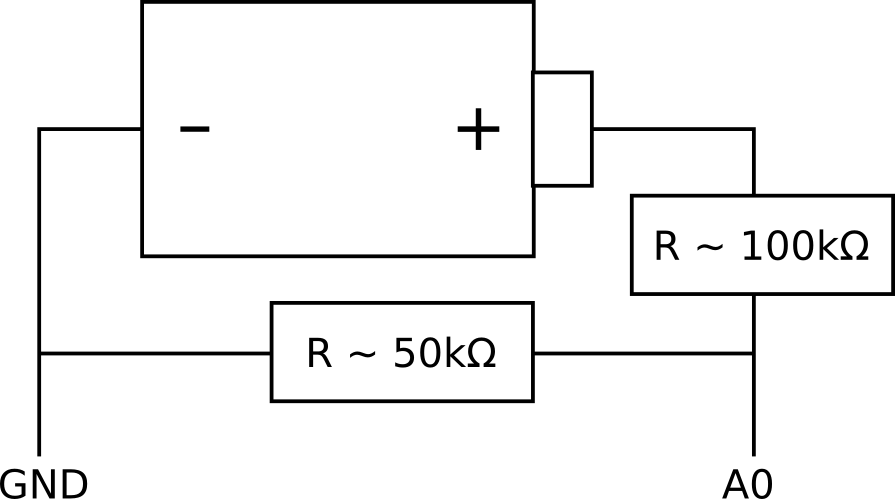
\includegraphics[width=0.65\textwidth]{latex/img/battery_scheme.png}
  \caption{The configuration needed to read battery level from pin A0.}\label{img:battery_scheme}
\end{figure}

\subsection{Resting}
The device can be put to rest when inactive. This can be done connecting \textbf{D0 to RST} and with the following code lines:
\begin{lstlisting}[language=C++]
#define SECONDS_DS(seconds)  ((seconds)*1000000UL)
ESP.deepSleep(SECONDS_DS(600), WAKE_RF_DEFAULT);  
\end{lstlisting}


\subsection{Complete code}
\lstinputlisting[language=C]{arduino/HX711_DHT11_wifi/HX711_DHT11_wifi/HX711_DHT11_wifi.ino}
